\documentclass{article}
\usepackage{fancyhdr}
\usepackage{amsmath,amssymb}
\usepackage{geometry}
\usepackage{datetime}
\usepackage{enumerate}
\usepackage{graphicx}

%Insert page formatting here
%\hoffset = -.5in
\voffset = -0.375in
%\textwidth = 6in
\textheight = 8in
\headheight = 24pt

\pagestyle{fancy}

\rhead{Peter Olson\\Student ID: $441666$}
\lhead{Math 3200\\Homework 1}
\chead{\today}
\cfoot{}

%\addtolength{\headwidth}{\marginparsep}
%\addtolength{\headwidth}{\marginparwidth}

%\renewcommand{\labelitemi}{$\diamond$}
\renewcommand{\implies}{\rightarrow}
\newcommand{\widespace}{\qquad \qquad \;}
\newcommand{\tret}{\\ \hline}
\newcommand{\fh}{\tfrac{1}{2}}
\newcommand{\deriv}[2]{\frac{d #1}{d #2}}
\newcommand{\pderiv}[2]{\frac{\delta #1}{\delta #2}}
\newcommand{\vr}{\vec{r}}
\newcommand{\at}{\text{ at }}

\begin{document}
	\section*{Exercise 4.34}
	
	Shmokahs. The data is reproduced following the R code.
	\begin{enumerate}[\ \ (a)\ ]
		\item Aggregate the data over age groups and calculate the overall death rates for smokers and nonsmokers. Which group has the higher death rate?
		\\\\
		\textbf{Answer:}  In simply calculating a blunt summation of the living and dead smokers and non-smokers and then finding the percentage thereof that have died, it's quite obvious that the non-smokers have a higher rate of mortality than the smokers. Reference Figure 1.\\\\
		\begin{tabular}{|l|c|c|}
			\hline 
			& Non-Smoking & Smoking \\ 
			\hline 
			Mortality & \textbf{31.4\%} & 22.6\% \\ 
			\hline 
		\end{tabular} 
		\item Now calculate the adjusted (for age) death rates for smokers and nonsmokers. Which group has the higher death rate?\\\\
		\textbf{Answer:}  Now that the statistics are weighted by age, it becomes clear that smokers have a much higher rate of mortality than in almost all but one age group. However, and this becomes more clear when looking at the graphical representation of this data in Figure 2, it seems that the age of the participants when they took the study was the greatest determining factor in their rate of survival.\\\\
		\begin{tabular}{|l|c|c|}
			\hline
			Age& Non-Smoking Mortality & Smoking Mortality \\
			\hline
			18-24 & 1.61\% & \textbf{3.63\%} \\
			\hline
			25-34 & \textbf{3.18\%} & 2.41\% \\
			\hline
			35-44 & 5.78\% & \textbf{12.8\%} \\
			\hline
			45-54 & 15.3\% & \textbf{20.7\%} \\
			\hline
			55-64 & 33.0\% & \textbf{39.0\%} \\
			\hline
			65-74 & 78.2\% & \textbf{80.5\%} \\
			\hline
			  75+ & \textbf{100\%} &\textbf{ 100\%} \\
			\hline
		\end{tabular}
		\item What does the fact that there were far fewer smokers in the higher age groups suggest about the effect of smoking? This exercise illustrates what can go wrong if a covariate (age) is correlated with the risk factor (smoking) and outcome variable (survival).\\\\
		\textbf{Answer:}  As identified above, age appears to be the strongest driving factor when trying to determine if a member of the survey is going to die or not. However, an observation that's interesting to make is that, relative to the number of smokers that died over the course of the survey, those that were over the age of 55 make up the lion's share of that number, with the biggest proportion of smoker deaths occurring to 65-74 year olds. Reference Figure 3. It seems that smoking is most dangerous for older people, perhaps with weaker bodies.
		\subsubsection*{Figure 1.}
		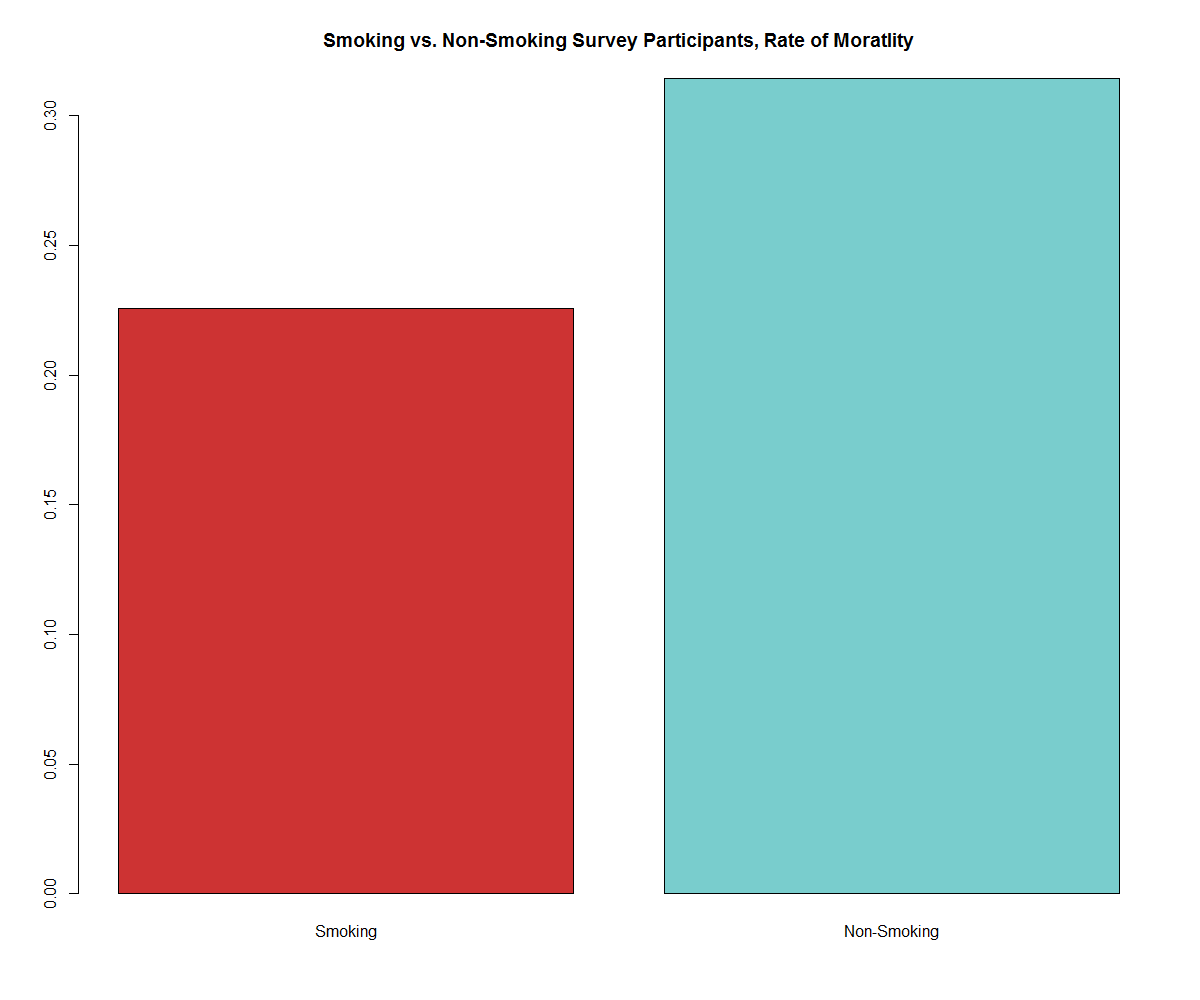
\includegraphics[width=4in]{P1.png}
		\subsubsection*{Figure 2.}
		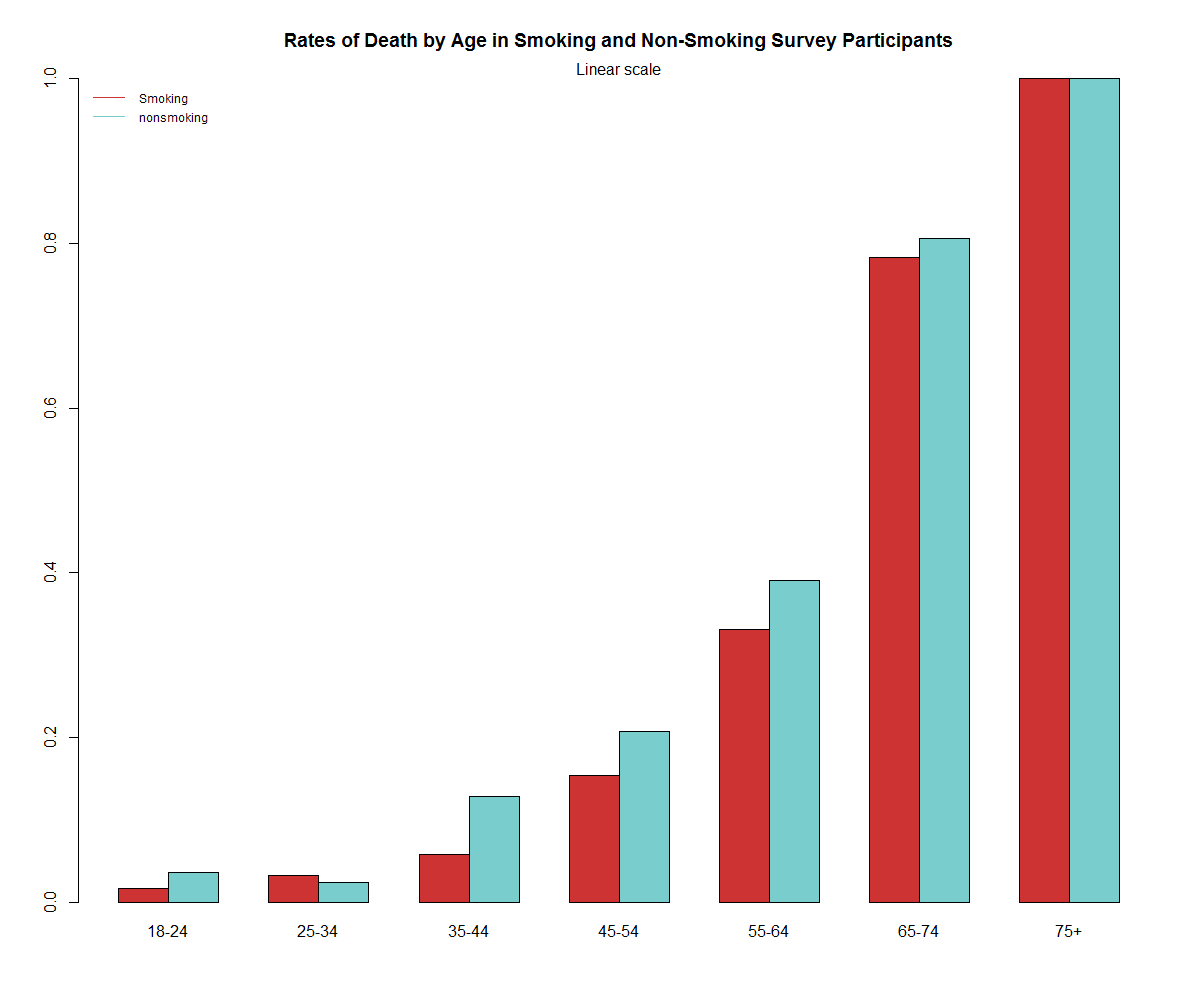
\includegraphics[width=4in]{P2.png}
		\subsubsection*{Figure 3.}
		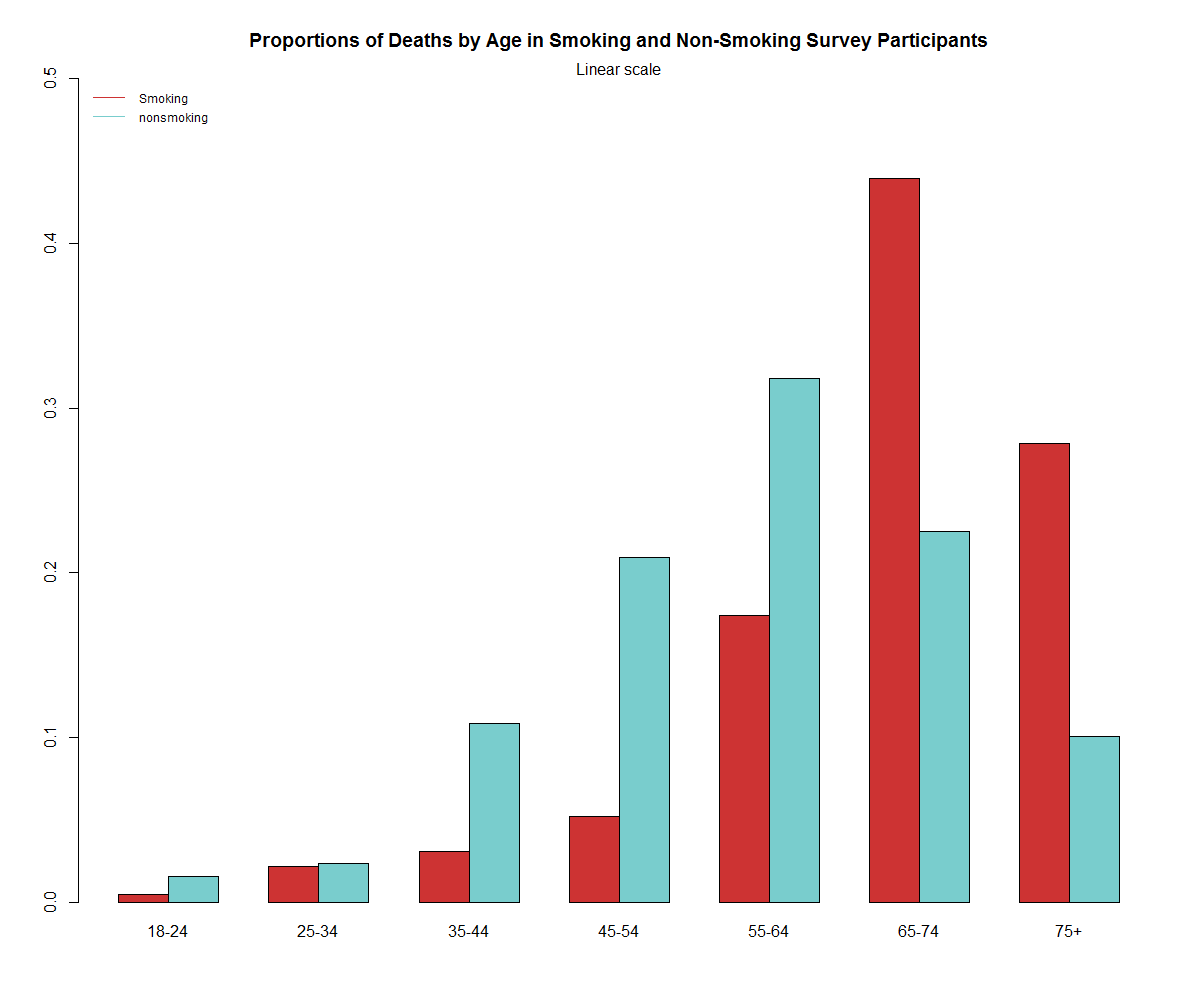
\includegraphics[width=4in]{P3.png}
		\subsection*{R Code}
		\begin{verbatim}
			#      Problem 6 - R Code
			# ==============================
			#     Author - Peter Olson
			#       Date - 2017-01-27
			#   Filename - SmokingKills.R
			# ==============================
			
			# Prepare data and dataframe
			
			lower_age = c(18, 25, 35, 45, 55, 65, 75)
			smokers_dead = c(2,3,14, 27, 41, 29, 13)
			smokers_alive = c(53, 121, 95, 103, 64, 7, 0)
			nonsmokers_dead = c(1, 5, 7, 12, 40, 101, 64)
			nonsmokers_alive = c(61, 152, 114, 66, 81, 28, 0)
			friendly_ages = c("18-24", "25-34", "35-44", "45-54", "55-64", "65-74", "75+")
			
			sm = data.frame(lower_age, nonsmokers_alive, nonsmokers_dead, smokers_alive, smokers_dead)
			
			total_smokers = (sum(smokers_alive) + sum(smokers_dead))
			total_nonsmokers = (sum(nonsmokers_alive) + sum(nonsmokers_dead))
			
			# Calculate an imprecise ratio for part 1
			
			s_blunt_ratio = sum(smokers_dead) / total_smokers
			n_blunt_ratio = sum(nonsmokers_dead) / total_nonsmokers
			
			# Used cat statement to get data for table in report
			#cat("Rate at which     smokers died:", s_blunt_ratio, "\n")
			#cat("Rate at which non-smokers died:", n_blunt_ratio, "\n")
			
			n_ratio = nonsmokers_dead / (nonsmokers_alive + nonsmokers_dead)
			s_ratio = smokers_dead / (smokers_alive + smokers_dead)
			# Used cat statement to get data for table in report
			# cat("Aged-rates of non-smokers:\n", n_ratio, "\nAged-rates of smokers:\n", s_ratio)
			
			# Matrix for first plot
			C = t(matrix(c(n_ratio, s_ratio), ncol = 2))
			#Matrix for second
			D = t(matrix(c(nonsmokers_dead/sum(nonsmokers_dead), smokers_dead/sum(smokers_dead)), ncol = 2))
			
			# Abbreviated theme
			theme = c("brown3", "darkslategray3")
			
			#
			# Figure 1
			#
			
			barplot(c(s_blunt_ratio, n_blunt_ratio),
			col = theme,
			main = "Smoking vs. Non-Smoking Survey Participants, Rate of Moratlity",
			names.arg = c("Smoking", "Non-Smoking")
			)
			
			#
			# Figure 2
			#
			
			barplot(C,
			main = "Rates of Death by Age in Smoking and Non-Smoking Survey Participants",
			col = theme, 
			ylim = c(0,1), 
			names.arg = friendly_ages,
			beside = TRUE)
			mtext("Linear scale")
			legend ('topleft', 
			legend=c("Smoking", "nonsmoking"),
			lty=1, col=theme,
			bty='n', 
			cex=.75)
			
			#
			# Figure 3
			#
			
			barplot(D,
			main = "Proportions of Deaths by Age in Smoking and Non-Smoking Survey Participants",
			col = theme, 
			ylim = c(0,0.5), 
			names.arg = friendly_ages,
			beside = TRUE)
			mtext("Linear scale")
			legend ('topleft', 
			legend=c("Smoking", "nonsmoking"),
			lty=1, col=theme,
			bty='n', 
			cex=.75)
			
		\end{verbatim}
	\end{enumerate}
\end{document}